% Created 2016-07-07 Thu 07:46
\documentclass[10pt,oneside,x11names]{article}
\usepackage[utf8]{inputenc}
\usepackage[T1]{fontenc}
\usepackage{fixltx2e}
\usepackage{graphicx}
\usepackage{grffile}
\usepackage{longtable}
\usepackage{wrapfig}
\usepackage{rotating}
\usepackage[normalem]{ulem}
\usepackage{amsmath}
\usepackage{textcomp}
\usepackage{amssymb}
\usepackage{capt-of}
\usepackage{hyperref}
\usepackage{geometry}
\usepackage{amsmath}
\usepackage{amssymb}
\usepackage{amsfonts}
\usepackage{palatino}
\usepackage{siunitx}
\usepackage{esdiff}
\usepackage{xfrac}
\usepackage{nicefrac}
\usepackage{faktor}
\usepackage[euler-digits,euler-hat-accent]{eulervm}
\author{Brian Beckman}
\date{\textit{<2016-05-03 Tue>}}
\title{Kalman Folding 7: A Small Streams Library (Review Draft)\\\medskip
\large Extracting Models from Data, One Observation at a Time}
\hypersetup{
 pdfauthor={Brian Beckman},
 pdftitle={Kalman Folding 7: A Small Streams Library (Review Draft)},
 pdfkeywords={},
 pdfsubject={},
 pdfcreator={Emacs 24.5.1 (Org mode 8.3.4)}, 
 pdflang={English}}
\begin{document}

\maketitle
\setcounter{tocdepth}{2}
\tableofcontents


\section{Abstract}
\label{sec:orgheadline1}

In \emph{Kalman Folding 5: Non-Linear Models and the EKF},\footnote{B. Beckman, \emph{Kalman Folding 5: Non-Linear Models and the EKF}, to appear.} we present an
Extended Kalman Filter as a fold over a lazy stream of observations that uses a
nested fold over a lazy stream of states to integrate non-linear equations of
motion. In \emph{Kalman Folding 4: Streams and Observables},\footnote{B. Beckman, \emph{Kalman Folding 4: Streams and Observables}, to appear.} we present a
handful of stream operators, just enough to demonstrate Kalman folding over
observables.

In this paper, we enrich the collection of operators, adding \emph{takeUntil},
\emph{last}, and \emph{map}. We then show how to use them to integrate differential
equations in state-space form in two different ways and to generate test cases
for the non-linear EKF from paper 5.

\section{Kalman Folding in the Wolfram Language}
\label{sec:orgheadline2}

In this series of papers, we use the Wolfram language\footnote{\url{http://reference.wolfram.com/language/}} because it
supports functional programming and it excels
at concise expression of mathematical code. All examples in these papers can be
directly transcribed to any modern mainstream language that supports closures.
For example, it is easy to write them in C++11 and beyond, Python, any modern
Lisp, not to mention Haskell, Scala, Erlang, and OCaml. Many can be written
without full closures; function pointers will suffice, so they are easy to write
in C. It's also not difficult to add extra arguments to simulate just enough
closure-like support in C to write the rest of the examples in that language.

\section{Review of Stream Basics}
\label{sec:orgheadline3}

From paper 4, we briefly review the following basics:

Represent a lazy stream as a pair, in curly braces, of a value and a \emph{thunk} (function of
no arguments).\footnote{This is quite similar to the standard --- not  Wolfram's --- definition of a list as a pair of a value and of another list.} The thunk must produce another lazy stream when called. Such
a stream can be infinite in abstract length because the elements of the stream are only
concretized in memory when demanded by calling thunks.

By convention, a finite stream has a \texttt{Null} thunk at the end. Thus, the empty
stream, obtained by invoking such a thunk, is \texttt{Null[]}, with empty square brackets
denoting invocation with no arguments.

A \emph{finite stream} is one that eventually produces \texttt{Null[]}.

One of Wolfram's notations for a literal thunk is an expression with an
ampersand at the end. An ampersand turns the expression to its left
into a thunk.

Here is a function that returns an infinite stream of natural numbers starting at \(n\):

\begin{verbatim}
integersFrom[n_Integer] := {n, integersFrom[n + 1] &}
\end{verbatim}

Calling, say, \texttt{integersFrom[42]} produces \texttt{\{42, integersFrom[42 + 1]\&\}}, a
stream consisting of an integer, \(42\), and another stream,
\texttt{integersFrom[42+1]\&}.

\section{Stream Operators}
\label{sec:orgheadline12}

The following are just sketches, suitable for research but not for release to
third-party users, who will need packaging, namespacing, documentation, and
error handling. In fact, it is easy to construct pathological cases that
circumvent the stated semantics for these implementations, which are designed
only to illustrate the concepts and to support the examples in this series of
papers. 

Furthermore, this is just a representative set found most useful while
developing Kalman folding, not anything like a complete set. It turns out that
nearly identical sets of operators can be developed for any kind of sequential
collection. Haskell\footnote{\url{http://learnyouahaskell.com/higher-order-functions}} has operators for lists, Rx\footnote{\url{http://introtorx.com/}} has a large
set for observables, and LINQ\footnote{LINQ's Standard Query Operators} has sets for many types including SQL
tables. Haskell also includes mechanisms\footnote{\url{https://en.wikipedia.org/wiki/Monad}}\textsuperscript{,}\,\footnote{See Haskell's type classes} for abstracting the
underlying collection, making it easy to implement a standardized set of
operators for any new, user-defined collection type.

\subsection{Extract :: Stream \(\rightarrow\) Value}
\label{sec:orgheadline4}

\emph{Extract} pulls the \(n\)-th element, \(1\)-indexed, from a given stream. Its run
time is \(O(n)\) and its space consumption is constant, \(O(1)\).

First, a base case. Extracting any element from the empty stream \texttt{Null[]}
should produce nothing, represented in Wolfram by \texttt{Null} without the brackets,
which conveniently does not print in a Mathematica notebook.

\begin{verbatim}
extract[Null[], _] := Null;
\end{verbatim}

Another base case is to get the first value from a stream. This overload
\emph{pattern-matches}\footnote{\url{http://tinyurl.com/j5jzy69}} or \emph{destructures} its stream input, instantiating the
variables \texttt{v} and \texttt{thunk} to the two components of that input. It then returns
the value \texttt{v}.

\begin{verbatim}
extract[{v_, thunk_}, 1] := v;
\end{verbatim}

The final, recursive case extracts the \(n-1\)-th element from the tail of the
input stream by discarding the current value \texttt{v} and invoking the \texttt{thunk}. This
runs in constant memory when the programming language supports tail-recursion,
as Wolfram does.\footnote{\url{https://en.wikipedia.org/wiki/Conditional_term_rewriting}} If the programming language does not, \texttt{extract} should be
implemented with a loop.

The notation \texttt{/;} precedes a conditional expression in the scope of the argument
list. In most other languages, this would be implemented by a conditional test
in the body of the function.

\begin{verbatim}
extract[{v_, thunk_}, n_Integer /; n > 1] := extract[thunk[], n - 1];
\end{verbatim}

Now we can get the 630000-th integer efficiently in space, if not terribly quickly:

\begin{verbatim}
Block[{$IterationLimit = Infinity},
  extract[integersFrom[1], 630000]] // AbsoluteTiming
~~>
{1.47735 second, 630000}
\end{verbatim}

Without tail recursion, this would exceed the system's stack depth.

\subsection{Disperse :: List \(\rightarrow\) Stream}
\label{sec:orgheadline5}

We'll need a way to convert a whole finite list into a stream.  There are three cases: an
empty list, a singleton list, and the inductive or recursive  case.

\begin{verbatim}
disperse[{}] := Null[]; (* empty list yields empty stream       *)
disperse[{x_}] := {x, Null}; (* the stream for a singleton list *)
disperse[{v_, xs__}] := {v, disperse[{xs}] &}; (* recursion     *)
\end{verbatim}

\subsection{Reify :: Stream \(\rightarrow\) List}
\label{sec:orgheadline6}

We need to go the other way, too; don't call this on an infinite stream:

\begin{verbatim}
reify[Null[]] := {};         (* produce empty list from empty stream *)
rify[{v_, Null}] := {v};     (* singleton list from singleton stream *)
reify[{v_, thunk_}] := Join[{v}, reify[thunk[]]]; (* recursion       *)
\end{verbatim}

\noindent \emph{Reify} undoes \emph{disperse}:

\begin{verbatim}
reify@disperse@{1, 2, 3}
~~> {1, 2, 3}
\end{verbatim}

\subsection{Take :: Stream \(\rightarrow\) FiniteStream}
\label{sec:orgheadline7}

Infinite streams are very important, but we frequently want finite subsets so
that we don't have to explicitly extract values by index. \emph{Take} takes a stream
and an element count and produces another stream that eventually yields
\texttt{Null[]}, that is, a finite stream. Because the streams are lazy, \emph{take} doesn't
actually run until elements are demanded, say by \emph{extract}, \emph{last}, or \emph{reify}. 

\begin{verbatim}
take[_, 0] := Null[];
take[Null[], _] := Null[];
take[{v_, thunk_}, 1] := {v, Null};
take[{v_, thunk_}, n_Integer /; n > 1] := {v, take[thunk[], n - 1] &};
\end{verbatim}

Produce a finite stream of three integers; extract the first value:

\begin{verbatim}
extract[take[integersFrom[1], 3], 1]
~~> 1
\end{verbatim}

\noindent and the last value:

\begin{verbatim}
extract[take[integersFrom[1], 3], 3]
~~> 3
\end{verbatim}

\noindent If we extract too far into a finite stream, we get \texttt{Null}, which doesn't print to the notebook:

\begin{verbatim}
extract[take[integersFrom[1], 3], 4]
~~>
\end{verbatim}

\subsection{TakeUntil :: Stream \(\rightarrow\) Predicate \(\rightarrow\) Stream}
\label{sec:orgheadline8}

\emph{TakeUntil} produces a new stream that produces elements from the original
stream, evaluating the predicate on them until it produces \texttt{True}, at which
point it permanently produces the empty stream \texttt{Null[]}.

\begin{verbatim}
takeUntil[Null[], _] := Null[];
takeUntil[{v_, thunk_}, predicate_] /; predicate[v] := Null[];
takeUntil[{v_, thunk_}, predicate_] := {v, takeUntil[thunk[], predicate] &};
\end{verbatim}

\begin{verbatim}
reify[takeUntil[integersFrom[1], # >= 3 &]]
~~> {1, 2, 3}
\end{verbatim}

\subsection{MapStream :: Stream \(\rightarrow\) UnaryFunction \(\rightarrow\) Stream}
\label{sec:orgheadline9}

\emph{MapStream} converts a stream into another stream of equal length by applying the
given unary function to the elements one at a time. Because it converts a lazy
stream to a lazy stream, it is safe to apply to infinite streams: nothing
happens until elements are demanded.

\begin{verbatim}
ClearAll[mapStream];
mapStream[Null[], _] := Null[];
mapStream[{v_, thunk_}, f_] := {f[v], mapStream[thunk[], f] &};
\end{verbatim}

Here we map the unary function \texttt{\#\textasciicircum{}2 \&}, which squares its single argument \texttt{\#},
over a finite sub-stream of the integers.

\begin{verbatim}
reify@mapStream[take[integersFrom[1], 3]]
~~> {1, 4, 9}
\end{verbatim}

\subsection{Last :: Stream \(\rightarrow\) Value}
\label{sec:orgheadline10}

\emph{Last} produces the last value in a finite stream without an
explicit index. It requires tail recursion to run in constant memory.

\begin{verbatim}
last[Null[]] := Null;
last[{v_, thunk_} /; thunk[] === Null[]] := v;
last[{v_, thunk_}] := last[thunk[]];
\end{verbatim}

Called on an empty stream, \emph{last} produces \texttt{Null}, which does not print.

\begin{verbatim}
last@disperse[{}]
~~>
\end{verbatim}

\noindent Otherwise, it produces the last element, even of a very long finite stream:

\begin{verbatim}
Block[{$IterationLimit = Infinity},
  last@take[integersFrom[1], 630000]] // AbsoluteTiming
~~> {4.72633 sec, 630000}
\end{verbatim}

\noindent The at-sign \texttt{@} is Wolfram's prefix form for function invocation;
\texttt{f@x} is the same as \texttt{f[x]}.

\subsection{foldStream}
\label{sec:orgheadline11}

Our equivalent for Wolfram's \emph{FoldList} is \emph{foldStream}.\footnote{The initial uncial (lower-case) letter signifies that \emph{we} wrote this function; it wasn't supplied by Wolfram.} Its type is similar

\begin{align*}
\text{foldStream :: }
\text{AccumulatorFunction}
\rightarrow
\text{Accumulation}\\
\rightarrow
\text{Stream}\left[\,\text{Observation}\,\right]
\rightarrow
\text{Stream}\left[\,\text{Accumulation}\,\right]
\end{align*}

\noindent Here is an implementation:

\begin{verbatim}
foldStream[f_, s_, Null[]] := (* acting on an empty stream *)
  {s, Null}; (* produce a singleton stream containing 's'  *)
foldStream[f_, s_, {z_, thunk_}] :=
  (* pass in a new thunk that recurses on the old thunk    *)
  {s, foldStream[f, f[s, z], thunk[]] &};
\end{verbatim}

\noindent and an example that produces the Fibonacci numbers in pairs:

\begin{verbatim}
allFibs = foldStream[
   Function[{s, z}, {s[[2]], s[[1]] + s[[2]]}],
   {0, 1},
   integersFrom[0]];

Transpose@reify@[take[allFibs, 11]]
~~>
\end{verbatim}
\(
\left(
\begin{array}{ccccccccccc}
 0 & 1 & 1 & 2 & 3 & 5 & 8 & 13 & 21 & 34 & 55 \\
 1 & 1 & 2 & 3 & 5 & 8 & 13 & 21 & 34 & 55 & 89 \\
\end{array}
\right)
\)

\section{EKF}
\label{sec:orgheadline13}

The EKF developed in paper 5 is

\begin{verbatim}
  EKFDrag[sigmaXi_, Zeta_, Phi_, Xi_, integrator_, fdt_, idt_]
   [{x_, P_}, {t_, A_, z_}] :=
   Module[{x2, P2, D, K},
    x2 = last[takeUntil[foldStream[integrator, {t, x},
         dragDStream[{idt, t, dragD}]],
        First[#] > t + fdt &]][[2]];
    P2 = sigmaXi^2 Xi[fdt, x] + Phi[fdt, x].P.Transpose[Phi[fdt, x]];
    D = Zeta + A.P2.Transpose[A];
    K = P2.Transpose[A].inv[D];
    {x2 + K.(z - A.x2), P2 - K.D.Transpose[K]}];
\end{verbatim}

\noindent The EKF integrates the equations of state evolution, which can be
arbitrarily nonlinear, by folding an integrator over a stream \texttt{dragDStream}. The
integrator operates on a time increment \texttt{idt}, which is often smaller than the
overall update period \texttt{fdt} of the EKF. The last element of the integrated
stream is collected and used as the state update for the filter.

The integrated stream advances time and passes through to the integrator a
function \texttt{Dx} that produces differential increments from the state and the time.
In our example, \texttt{Dx} is \texttt{dragD}, which computes the height \texttt{x} of an object
falling at speed \texttt{v} and experiencing aerodynamic drag. Don't confuse this \texttt{x}
with the vector \texttt{x} that represents the state in the integrators. It's difficult
not to run out of symbols.

\begin{verbatim}
  dragDStream[Delta : {dt_, t_, Dx_}] :=
    {Delta, dragDStream[{dt, t + dt, Dx}] &};
  dragD[{x_, v_}, t_] := {v, g (A Exp[-x/k] v^2/(2. beta) - 1)};
\end{verbatim}

The additional functions \texttt{Phi} and \texttt{Xi} use linear approximations of the
equations of state evolution to advance the gain \texttt{K} and the covariance \texttt{P}.
They are explained in paper 5.

The simplest integrator is the Euler integrator, which updates a state with its
derivative times a small interval of time. This is a binary function, like all
accumulator functions for folds, that takes an accumulation and an observation
and produces a new accumulation. In our case, the accumulation is a pair of a
scalar time \texttt{t} and a vector state \texttt{x}, and the observation is a triple of a
time increment \texttt{dt}, a time \texttt{t}, and the function \texttt{Dx} that produces
differential increments.

\begin{verbatim}
eulerAccumulator[{t_, x_}, {dt_, t_, Dx_}] :=
  {t + dt, x + dt Dx[x, t]};
\end{verbatim}

Much better numerics can be achieved with the Runge-Kutta integrators, which are
drop-in replacements for the Euler integrator at the cost of calling \texttt{Dt} more often:

\begin{verbatim}
rk2Accumulator[{t_, x_}, {dt_, t_, Dx_}] :=
  With[{dx1 = dt Dx[x, t]},
   With[{dx2 = dt Dx[x + .5 dx1, t + .5 dt]},
    {t + dt, x + (dx1 + dx2)/2.}]];
rk4Accumulator[{t_, x_}, {dt_, t_, Dx_}] :=
  With[{dx1 = dt Dx[x, t]},
   With[{dx2 = dt Dx[x + .5 dx1, t + .5 dt]},
    With[{dx3 = dt Dx[x + .5 dx2, t + .5 dt]},
     With[{dx4 = dt Dx[x + dx3, t + dt]},
      {t + dt, x + (dx1 + 2. dx2 + 2. dx3 + dx4)/6.}]]]];
\end{verbatim}

\section{Testing the EKF}
\label{sec:orgheadline14}

We test the EKF by folding it over another lazy stream --- a stream of
observation packets \texttt{\{t, A, z\}} of time \texttt{t}, model partial derivatives \texttt{A}, and
observations \emph{per-se} \texttt{z}. Unlike the filter itself, the test code does not run
in constant memory. It doesn't have to --- its purpose is to assist the
verification of the filter by creating sample data, statistics, and plots. It
does so by reifying some finite substreams of infinite streams.

First, we set up some constants

\begin{verbatim}
With[{nStates = 2, nIterations = 10},
 With[{sigmaZeta = 25., sigmaXi = 0.0, t0 = 0., t1 = 30., 
   filterDt = 0.1, integrationDt = 0.1},
  With[{x0 = 200000, v0 = -6000, Zeta = sigmaZeta^2 id[1], 
    P0 = 1000000000000 id[nStates]},
\end{verbatim}

\noindent We then build some fake data by building a lazy stream that integrates
the equations of motion, producing an infinite stream of time-state pairs
starting with \texttt{\{t0, \{x0, v0\}\}}, where \texttt{t0} is the initial scalar time and \texttt{\{x0,
v0\}} is the initial vector state:

\begin{verbatim}
   Module[{fakes},
    fakes[] := foldStream[rk4Accumulator, {t0, {x0, v0}},
      dragDStream[{filterDt, t0, dragD}]];
\end{verbatim}

\begin{figure}[htb]
\centering
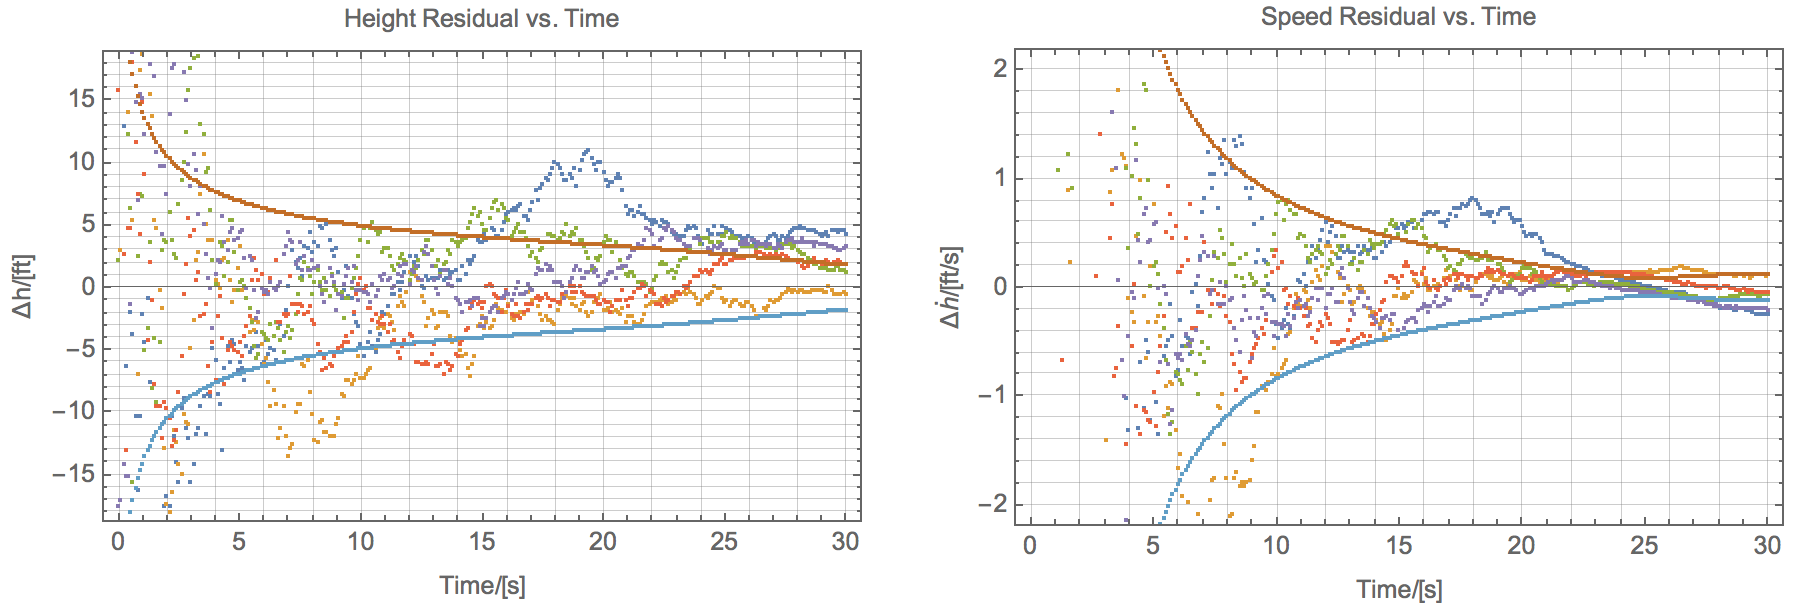
\includegraphics[width=.9\linewidth]{rk2-idt-point-001-zeta-25.png}
\caption{\label{fig:orgparagraph1}
RK-2 integrator, \texttt{idt} \(= 0.001\) sec, \(\sigma_\zeta = 25\) ft; also RK-4 integrator, \texttt{idt} \(= 0.1\) sec}
\end{figure}

\noindent We now set up some variables to hold the results of multiple
iterations of the integration. We use these variables to produce the statistical
plots in paper 5, one of which we reproduce here in figure
\ref{fig:orgparagraph1}. 
The variables are:
\begin{description}
\item[{\texttt{ffs}}] a finite substream of the fakes, pairs of times and states
\item[{\texttt{rffs}}] an array: the reification of \texttt{ffs}
\item[{\texttt{ts}}] an array of times gotten by mapping the function \texttt{pick[1]} over \texttt{rffs}
     using Wolfram's built-in mapping operator \texttt{/@} for reified lists.
\item[{\texttt{txs}}] an array of ground-truth values for the first state component \texttt{x},
the height of the falling object, for computing residuals
\item[{\texttt{tvs}}] an array of ground-truth values for the second state component \texttt{v},
the speed of the falling object, for computing residuals
\item[{\texttt{xss}, \texttt{vss}}] parallel arrays of arrays of heights and speeds. The outer
array has length \texttt{nIterations} and is built by mapping (using Wolfram's
built-in \texttt{Map}) a function over \texttt{Range[nIterations]}, a
list of the integers \(1, 2, \ldots, \texttt{nIterations}\). The inner arrays have the
same length as \texttt{ts}, for plotting. These can be fed straight into Wolfram's
plotting functions.
\item[{\texttt{xvs}, \texttt{ps}}] parallel arrays of vector states \texttt{\{x, v\}} and covariance
matrices gotten by folding the EKF over a stream built by \texttt{mapStream}-ing a
function over the finite fakes stream \texttt{ffs}. That function picks the times
(from the first element of its argument \texttt{\#} via
\texttt{\#}\(\left[\left[1\right]\right]\)) and the heights (from element \(2, 1\) its argument \texttt{\#} via
\texttt{\#}\(\left[\left[2,1\right]\right]\)) from the finite fakes
\texttt{ffs} and builds a stream of observation packets with the constant,
\(1\times{2}\) matrix \(\mathbold{A}=\texttt{\{\{1, 0\}\}}\).
\end{description}

\begin{verbatim}
    SeedRandom[44];
    Module[{ffs, rffs, ts, txs, tvs, xss, vss, xvs,
      ps, sigmaxs, sigmavs},
     xss = ConstantArray[0, nIterations];
     vss = ConstantArray[0, nIterations];
     ffs = takeUntil[fakes[], First@# > t1 &];
     rffs = reify@ffs;
     ts = pick[1] /@ rffs;
     txs = pick[2, 1] /@ rffs;
     tvs = pick[2, 2] /@ rffs;
     {xss, vss} = Transpose@Map[
        ({xvs, ps} = Transpose@Rest@reify@foldStream[
               EKFDrag[sigmaXi, Zeta, Phi, Xi,
                 rk4Accumulator, filterDt, integrationDt],
               {{0, 0}, P0},
               mapStream[ffs,
                 {#[[1]], { {1, 0} }, #[[2, 1]] + gen[Zeta]} &]];
          sigmaxs = Sqrt[pick[1, 1] /@ ps;
          sigmavs = Sqrt[pick[2, 2] /@ ps;
          Transpose@xvs) &,
        Range[nIterations]];
\end{verbatim}

Some minor manipulation of these arrays suffice to produce a plot like figure 
\ref{fig:orgparagraph1}.

This test harness uses many of the stream operators in the little library,
namely \texttt{takeUntil}, \texttt{reify}, \texttt{foldStream}, and \texttt{mapStream}, but the EKF does not
know and cannot detect that it's being called through lazy streams. This is one
of the secrets of Kalman folding that allows code to be tested in one
environment and moved verbatim into other environments. It's even feasible to
change integrators at run time through a functional shim. The only thing EKF
knows is that it's internally stream-folding an integrator provided by its caller
through a fixed interface contract.

\section{Concluding Remarks}
\label{sec:orgheadline15}

Lazy infinite streams are one of the kinds of collections supported by Kalman
folding. They afford space-efficient integration of differential equations, but
also concise and elegant test fixtures. As with all Kalman-folding scenarios,
the code-under-test can be moved verbatim, without even recompilation, from the
test environment to production and embedded environments.
\end{document}